% =============================================================================
%  Chapitre 4 — Modélisation et protocole d'évaluation
%
%  Ce chapitre décrit ce qui a été construit et comment il est jugé ; il ne
%  donne aucun résultat chiffré, qui font l'objet du chapitre 5. La séparation
%  est délibérée : le protocole doit pouvoir être lu — et critiqué — avant de
%  connaître les conclusions qu'il produit.
% =============================================================================

\chapter{Modélisation et protocole d'évaluation}
\label{chap:modelisation}

\section*{Ce que ce chapitre explique}
\addcontentsline{toc}{section}{Ce que ce chapitre explique}

Le chapitre précédent a décrit la chaîne qui produit les données et le moteur
qui exécute les stratégies. Celui-ci décrit \emph{les stratégies elles-mêmes} —
quatre familles de modèles, construites l'une après l'autre — puis le dispositif
qui décide si elles valent quelque chose.

Ce chapitre ne contient volontairement \textbf{aucun résultat chiffré}. Le
protocole d'évaluation doit pouvoir être lu, compris et contesté indépendamment
des conclusions qu'il produit~; si les deux étaient présentés ensemble, un
lecteur ne pourrait plus distinguer un protocole conçu pour être juste d'un
protocole conçu pour donner raison. Les chiffres sont au
chapitre~\ref{chap:resultats}.

Deux principes de méthode gouvernent tout ce qui suit.

\textbf{Une seule chose change à la fois.} Les modèles sont ajoutés par
\emph{échelons}, chacun ne modifiant qu'un ingrédient du précédent. Un gain
devient alors attribuable~: on sait \emph{à quoi} il est dû. C'est le contraire
de la démarche qui consiste à assembler d'emblée le système le plus sophistiqué
possible et à constater qu'il fonctionne, sans pouvoir dire pourquoi.

\textbf{Rien ne touche au moteur.} Toutes les stratégies décrites ci-dessous
respectent la même interface~: elles reçoivent une fenêtre d'entraînement et
retournent une répartition. Aucune n'a nécessité de modifier le moteur de
backtest ni ses garanties. C'est ce qui rend leurs performances comparables~:
elles ont été mesurées par le même instrument, sans exception.

% =============================================================================
\section{Les références classiques}
% =============================================================================

Quatre stratégies non--ML servent de référence. Elles ne sont pas un
échauffement~: ce sont les concurrentes que le ML doit battre, et l'une d'elles
est notoirement difficile à battre.

\begin{itemize}
  \item \textbf{L'équipondération} — la même somme sur chaque actif. Aucun
        paramètre, aucune estimation, donc aucune erreur d'estimation
        possible. La littérature établit qu'elle bat, une fois les coûts
        déduits, la plupart des optimiseurs~; c'est la référence honnête par
        excellence.
  \item \textbf{La variance minimale} — la répartition qui minimise la
        volatilité du portefeuille, sans chercher à prévoir les rendements.
  \item \textbf{La variance minimale à covariance rétrécie} — la même, avec la
        correction d'estimation décrite plus bas.
  \item \textbf{Le Markowitz classique} (Sharpe maximal) — la formulation de
        1952~: on maximise le rendement attendu par unité de risque, en
        estimant les rendements attendus par leur moyenne historique.
\end{itemize}

Toutes s'exécutent sous les contraintes réelles décrites au
chapitre~\ref{chap:architecture} — pas de vente à découvert, plafond de 25~\%
par actif, coûts de transaction déduits — et sur les deux univers.

% =============================================================================
\section{Premier échelon : mieux estimer le risque (P1)}
% =============================================================================

Le problème P1 est celui de l'\emph{erreur d'estimation}. La matrice de
covariance — qui décrit comment les actifs bougent ensemble — doit être estimée
à partir d'un échantillon fini. Avec neuf actifs, elle comporte 45~quantités
distinctes à estimer~; chacune est bruitée, et l'optimiseur, qui cherche
l'extremum, se précipite précisément sur les combinaisons où le bruit lui est
favorable. Il produit alors un portefeuille concentré, magnifique sur le passé et
fragile sur l'avenir.

Quatre échelons ont été construits, du plus simple au plus élaboré.

\begin{enumerate}
  \item \textbf{Covariance empirique} — la moyenne des co-mouvements observés.
        Le point de départ, et le plus exposé au bruit.
  \item \textbf{Rétrécissement de Ledoit-Wolf} — on mélange la matrice observée
        avec une matrice « naïve » très structurée, dans une proportion
        calculée automatiquement. On accepte un biais volontaire contre une
        forte réduction de variance. C'est le compromis classique de la
        statistique~: une estimation légèrement fausse mais stable bat une
        estimation juste en moyenne mais instable.
  \item \textbf{Covariance à mémoire exponentielle} — les observations récentes
        pèsent davantage que les anciennes, avec une décroissance géométrique.
        C'est la première réponse au problème P2~: si le marché change de
        régime, l'année dernière est plus informative que la précédente.
  \item \textbf{DCC-GARCH} — le modèle le plus élaboré de la chaîne. Il estime
        d'abord, actif par actif, un modèle de volatilité variable dans le
        temps (les fortes secousses en appellent d'autres, phénomène bien
        documenté), puis fait évoluer les \emph{corrélations} elles-mêmes selon
        leur propre dynamique.
\end{enumerate}

\begin{remarquebox}
Le quatrième échelon a demandé un travail d'implémentation réel~: la
bibliothèque employée fournit uniquement des modèles de volatilité
\emph{univariés}. La récursion multivariée d'Engle (2002) et l'estimation de ses
deux paramètres par maximum de vraisemblance ont donc été écrites à la main. Une
sécurité l'accompagne~: si l'estimation ne converge pas pour un actif, la
stratégie retombe sur le rétrécissement de Ledoit-Wolf en journalisant un
avertissement. Ce filet s'est déclenché une fois en conditions réelles, sur une
seule fenêtre et un seul actif — le dispositif fonctionne, et il ne fonctionne
pas seulement dans les tests.
\end{remarquebox}

% =============================================================================
\section{Deuxième échelon : reconnaître le régime de marché (P2, P3)}
% =============================================================================

\begin{definitionbox}{Modèle de Markov caché}
Modèle statistique supposant que les observations (ici~: rendement du marché,
volatilité récente, corrélation moyenne entre actifs) sont engendrées par un
\emph{état} non observable qui change au cours du temps. On ne voit jamais l'état
directement~; on l'infère à partir de ce qu'il produit. Le modèle est
\emph{non supervisé}~: on ne lui fournit aucune liste de crises, il découvre
lui-même que deux régimes de comportement coexistent.
\end{definitionbox}

Le détecteur est entraîné sur trois variables seulement — le rendement du
marché, sa volatilité récente et la corrélation moyenne entre actifs. Ce choix
est directement dicté par les problèmes~: la volatilité est la signature de P2,
la corrélation moyenne est la mesure même de P3. À chaque décision, le modèle
est réentraîné sur la seule fenêtre disponible et produit une probabilité de
régime (figure~\ref{fig:regimes}).

\begin{figure}[htbp]
  \centering
  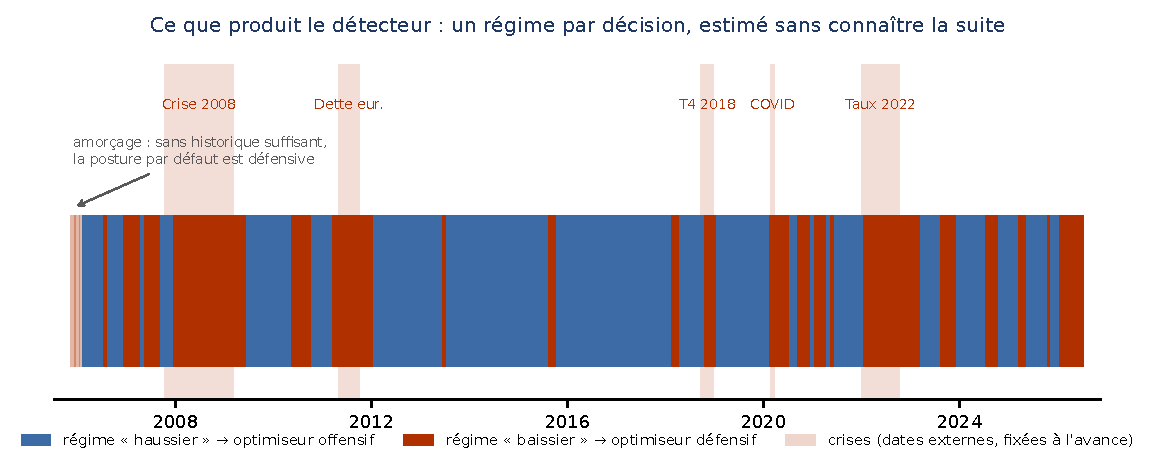
\includegraphics[width=\textwidth]{assets/figures/regimes_timeline.pdf}
  \caption[Sortie du détecteur de régime]{Sortie du détecteur sur l'univers ETF~:
  un régime par décision de rééquilibrage, estimé sans aucune connaissance de la
  suite. Les bandes verticales marquent cinq crises dont les dates proviennent
  d'une source externe et ont été fixées \emph{avant} toute mesure. La question
  de savoir si les amas rouges coïncident significativement avec ces bandes est
  traitée au chapitre~\ref{chap:resultats}.}
  \label{fig:regimes}
\end{figure}

Quatre décisions de conception méritent d'être justifiées, car elles ont toutes
été prises contre l'option en apparence plus ambitieuse.

\textbf{Deux états, pas trois.} Un troisième état « crise » était tentant. Il a
été écarté parce que l'univers principal ne compte qu'environ 1\,300~journées~:
un troisième état aurait été estimé sur une poignée d'observations, et sa
définition aurait dépendu de la graine aléatoire plus que des données.

\textbf{Un basculement franc, pas un mélange.} Une fois le régime identifié, la
décision est entièrement confiée à une stratégie classique déjà testée~: le
Markowitz classique en régime haussier, la variance minimale rétrécie en régime
baissier. Aucun code d'optimisation nouveau n'a été écrit. L'inconvénient est
assumé et documenté~: un basculement franc provoque un pic de transactions à la
frontière entre deux régimes, et c'est effectivement la stratégie la plus
coûteuse en rotation du projet.

\textbf{En cas de doute, la posture défensive.} Si la fenêtre est trop courte ou
si l'estimation ne converge pas, la probabilité neutre de 50/50 est résolue vers
la stratégie \emph{défensive}, non vers un tirage arbitraire. Un système
d'allocation qui ne sait pas où il est ne doit pas parier à la hausse.

\textbf{Les étiquettes sont recalculées à chaque réestimation.} La bibliothèque
employée ne garantit pas que l'état numéro~0 désigne le même régime d'une
estimation à l'autre. Les états sont donc réordonnés à chaque fois d'après le
rendement moyen ajusté, et « baissier » est \emph{défini} comme l'état de
rendement moyen le plus faible. Cette définition a une conséquence importante,
rappelée au chapitre~\ref{chap:resultats}~: une partie de l'association entre
régime baissier et crise est définitionnelle, et seul le caractère
\emph{temps réel} de la détection est un résultat.

% =============================================================================
\section{Troisième échelon : prédire les rendements}
% =============================================================================

Les échelons précédents ne prédisent jamais un rendement~: ils estiment un
risque et un régime. L'échelon suivant franchit ce pas — c'est la fonction que
le référentiel fonctionnel d'EURAFRIC désigne comme « modèles ML adaptatifs ».

Deux familles ont été retenues, toutes deux fondées sur des ensembles d'arbres de
décision~: forêts aléatoires et gradient boosting. Aucun réseau de neurones n'a
été conservé — un modèle récurrent avait été développé et testé isolément, puis
retiré de la comparaison après un conflit reproductible entre deux bibliothèques
natives chargées dans le même processus. Il a paru préférable de retirer un
composant instable que de publier une comparaison qui n'aurait pas pu être
rejouée.

Trois choix structurent cette partie.

\textbf{Un modèle unique, entraîné sur tous les actifs à la fois.} Plutôt que
neuf modèles indépendants, un seul apprend sur un tableau où chaque ligne est un
couple (date, actif) et où l'identité de l'actif est une variable comme une
autre. L'intérêt est arithmétique~: le nombre de lignes d'entraînement est
multiplié par le nombre d'actifs. Sur un univers de 1\,300~journées, c'est la
différence entre un problème d'apprentissage difficile et un problème
impossible.

\textbf{Le régime est une variable d'entrée, pas un aiguillage.} La probabilité
de régime issue du détecteur est fournie au modèle comme une colonne
supplémentaire. L'alternative — deux modèles distincts, un par régime —
fragmenterait un jeu de données déjà mince pour un problème d'apprentissage plus
difficile que celui du détecteur.

\textbf{La prédiction remplace un seul ingrédient.} Le rendement prédit se
substitue à la moyenne historique dans l'objectif de Markowitz, déjà écrit et
déjà testé. La covariance reste inchangée. Le principe « une seule chose change
à la fois » est ainsi préservé jusqu'au bout~: tout écart de performance
s'attribue à la qualité de la prédiction, à rien d'autre.

\begin{remarquebox}
C'est ici que le risque de fuite est le plus grand, car la variable à prédire est
construite à partir de la même matrice de rendements que les variables
explicatives. La date de décision est donc exclue de l'entraînement
\emph{structurellement}, par comparaison de dates — et non par filtrage des
valeurs manquantes, qu'un appel maladroit pourrait contourner. Un test dédié
corrompt le futur et vérifie qu'aucune décision passée ne change, en s'assurant
au passage que le modèle utilise réellement ces variables~: sans cette seconde
vérification, la garantie serait vide.
\end{remarquebox}

% =============================================================================
\section{Quatrième échelon : payer le prix des transactions}
% =============================================================================

L'échelon précédent a produit un diagnostic précis, exposé au
chapitre~\ref{chap:resultats}~: le signal était informatif \emph{avant} coûts et
ne l'était plus après. Autrement dit, un échec de \emph{construction} de
portefeuille et non de \emph{prédiction}. Trois leviers ont été ajoutés en
réponse.

\textbf{Une pénalité de rotation.} L'objectif d'optimisation intègre un terme
proportionnel à l'ampleur des transactions envisagées~: la stratégie ne modifie
une position que si le gain attendu dépasse le coût du mouvement. Un détail
technique mérite mention, car il illustre le soin requis~: la valeur absolue
n'est pas dérivable exactement là où se situe l'optimum d'un problème pénalisé —
c'est-à-dire « ne rien échanger » — et l'algorithme employé est fondé sur le
gradient. Une approximation lisse de la valeur absolue est donc utilisée.

\textbf{Un rétrécissement des rendements prédits} vers la moyenne historique, et
une variante n'en conservant que le \emph{classement}. La justification est un
résultat classique~: une erreur sur les rendements attendus dégrade un
optimiseur moyenne-variance environ dix fois plus qu'une erreur équivalente sur
la covariance. Réduire l'amplitude d'une prédiction bruitée tout en conservant sa
direction est donc souvent préférable à s'y fier pleinement.

\textbf{Le choix de l'estimateur de covariance} devient un paramètre des
stratégies à signal, ce qui permet d'associer « meilleure prédiction » et
« meilleure covariance » par configuration plutôt que par écriture de code.

Tous ces leviers sont \textbf{désactivés par défaut}. La raison est de
reproductibilité~: l'échelon précédent, avec son résultat négatif, reste
exécutable à l'identique et sert de plancher honnête. On n'améliore pas un
résultat en le rendant irretrouvable.

% =============================================================================
\section{Le protocole d'évaluation (P4)}
% =============================================================================

Tout ce qui précède serait sans valeur si la mesure était complaisante. Le
problème P4 — le surapprentissage du backtest — est le seul des quatre qui ne
puisse pas être résolu par un meilleur modèle, puisqu'il porte sur la mesure
elle-même. Quatre dispositifs y répondent.

\subsection{Rejouer le temps}

Toute performance rapportée provient d'une simulation à fenêtre glissante
(figure~\ref{fig:walkforward})~: à chaque fin de mois, le modèle est réentraîné
sur les seules données antérieures, décide, puis subit le mois suivant. Aucune
performance n'est jamais mesurée sur des données ayant servi à décider.

\begin{figure}[htbp]
  \centering
  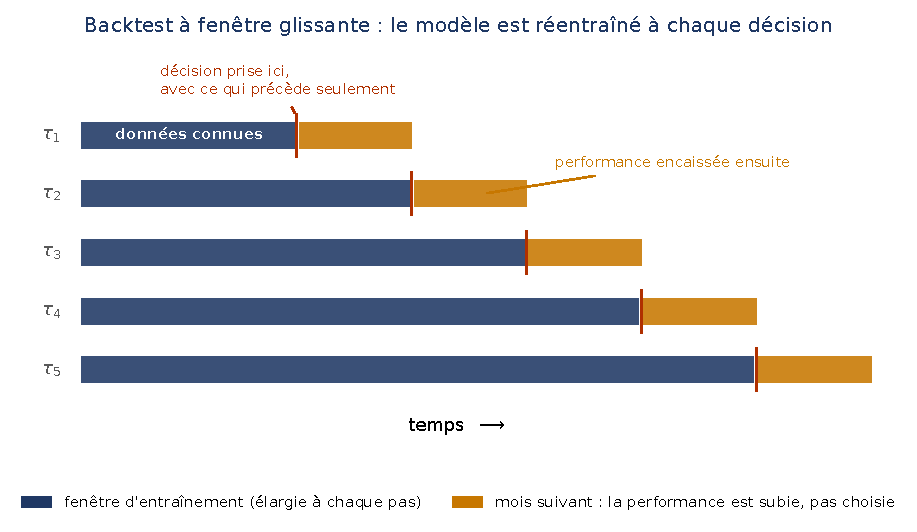
\includegraphics[width=0.94\textwidth]{assets/figures/walkforward.pdf}
  \caption[Backtest à fenêtre glissante]{Principe du backtest à fenêtre
  glissante. La fenêtre d'entraînement s'élargit à chaque pas~; la performance
  est toujours encaissée \emph{après} la décision. Le découpage est effectué par
  le moteur, jamais par la stratégie.}
  \label{fig:walkforward}
\end{figure}

\subsection{Choisir les hyperparamètres sans tricher}

Reste une fuite plus subtile~: le choix des réglages. Essayer trente
configurations et publier la meilleure revient à publier un maximum de bruit.

\begin{definitionbox}{Validation croisée purgée et sous embargo}
En apprentissage classique, on découpe les données en blocs et on teste sur
chacun à tour de rôle. Sur des séries temporelles financières, c'est fautif~: les
observations voisines se ressemblent, et la variable à prédire d'une journée
recouvre les journées suivantes. Le bloc de test « touche » donc son propre
entraînement. La \emph{purge} retire les observations d'entraînement dont
l'horizon chevauche le bloc de test~; l'\emph{embargo} écarte en outre une bande
de journées juste après ce bloc.
\end{definitionbox}

\begin{figure}[htbp]
  \centering
  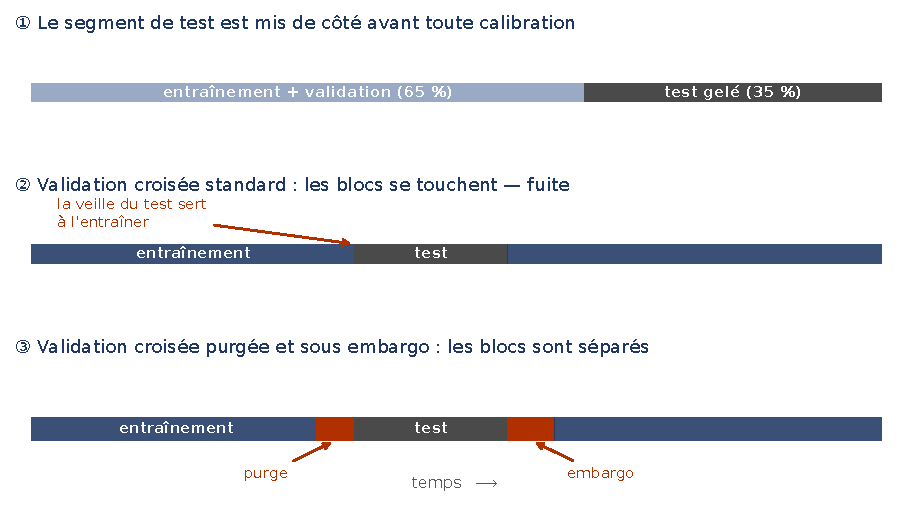
\includegraphics[width=0.94\textwidth]{assets/figures/validation_purgee.pdf}
  \caption[Protocole de sélection]{Le protocole de sélection. Le segment de test
  final est mis de côté avant toute calibration~; la sélection s'opère sur le
  reste, avec des blocs séparés par une purge et un embargo. Le découpage est
  effectué \emph{par date}, non par ligne, car le tableau d'apprentissage
  comporte plusieurs actifs à chaque date.}
  \label{fig:validation}
\end{figure}

Cette validation croisée a été implémentée dans le projet plutôt qu'importée~: la
bibliothèque spécialisée de référence a adopté un modèle de licence restrictif,
et une cinquantaine de lignes suffisaient. Un test de fuite dédié doit être vert
avant que quoi que ce soit ne l'utilise.

\subsection{Deux objectifs, deux instruments}

Une distinction, discrète mais décisive, structure la sélection.

\begin{definitionbox}{Coefficient d'information}
Corrélation de rang entre les rendements prédits et les rendements réalisés. Il
mesure si le modèle classe correctement les actifs — ce qui est exactement ce
qu'un signal doit faire — sans exiger que ses prédictions soient justes en
niveau. En prévision financière, un coefficient de quelques centièmes est déjà
considéré comme exploitable~; c'est un domaine où le signal est ténu par nature.
\end{definitionbox}

Les \emph{hyperparamètres des modèles} sont donc choisis par validation croisée
purgée, au coefficient d'information. Les \emph{leviers de portefeuille}
(rétrécissement, pénalité de rotation) sont choisis autrement~: sur un segment de
validation distinct, au ratio de Sharpe net, à travers le moteur réel — car ce
sont des paramètres de construction, pas de prédiction, et les juger au
coefficient d'information serait une erreur de catégorie.

\subsection{Un verdict rendu une seule fois, avec sa marge d'erreur}

Les derniers 35~\% de chaque univers sont mis de côté avant toute calibration et
ne sont utilisés qu'une fois, les réglages figés. À ce verdict s'ajoutent deux
précautions.

\begin{definitionbox}{Intervalle de confiance par bootstrap à blocs}
Pour estimer de combien une performance mesurée pourrait varier par simple
hasard, on reconstitue des milliers d'historiques fictifs en retirant au sort des
\emph{blocs} de journées consécutives — ici des blocs d'un mois environ, afin de
préserver la structure temporelle des rendements, qu'un tirage journée par
journée détruirait. La dispersion des performances obtenues donne l'intervalle.
\end{definitionbox}

\begin{definitionbox}{Ratio de Sharpe déflaté}
Probabilité qu'une performance mesurée soit réellement positive une fois
corrigée du nombre de stratégies essayées et de la non-normalité des rendements.
Essayer 200~configurations et retenir la meilleure produit une bonne performance
même si aucune ne vaut rien~; cette mesure quantifie cet effet.
\end{definitionbox}

Le nombre de configurations essayées n'est pas déclaré à la main~: un registre
enregistre chaque configuration évaluée pendant la recherche, et c'est ce
décompte qui alimente la correction. C'est une manière de rendre coûteuse — et
visible — la tentation d'essayer une piste de plus.

% =============================================================================
\section{La discipline expérimentale}
% =============================================================================

Trois règles de conduite complètent le dispositif technique. Elles ne relèvent
pas de l'outillage mais de l'honnêteté, et ce sont elles qui rendent le
chapitre~\ref{chap:resultats} défendable.

\textbf{Choisi n'est pas calibré.} Lorsqu'une valeur a été fixée par jugement et
non par une procédure de sélection, le rapport le dit. Ajuster ces valeurs en
regardant le résultat final serait exactement le surapprentissage que tout le
chapitre cherche à empêcher.

\textbf{Les issues sont écrites avant l'expérience.} Les études exploratoires du
projet énoncent, dans le script lui-même et avant exécution, les conclusions
associées à chaque issue possible — « si tel écart dépasse tel seuil, alors
l'hypothèse est retenue~; sinon elle est rejetée ». Plusieurs comportent en outre
un \emph{contrôle inversé}~: une variante délibérément construite à contresens,
qui doit faire moins bien. Si elle fait aussi bien, ce n'est pas l'hypothèse qui
est validée, c'est l'expérience qui est sans pouvoir.

\textbf{Un seuil ne se durcit qu'avant de voir le résultat.} Un exemple concret
mérite d'être rapporté, car il est plus parlant qu'un principe. Une expérience
comparait deux configurations avec un simple « meilleur que »~; un essai
préliminaire a rendu un écart de $+0{,}0016$, que cette règle aurait qualifié de
victoire. Un seuil de matérialité a donc été ajouté \emph{avant} l'exécution
réelle~; il rend le test plus sévère, et le changement est consigné dans le
script comme dans le document d'analyse plutôt que fondu silencieusement dans la
méthode.

% =============================================================================
\section*{Synthèse du chapitre}
\addcontentsline{toc}{section}{Synthèse du chapitre}

\begin{itemize}
  \item Quatre échelons ont été construits, chacun ne modifiant qu'un ingrédient
        du précédent~: meilleure estimation du risque (P1), reconnaissance du
        régime de marché (P2, P3), prédiction des rendements, puis prise en
        compte du coût des transactions. Un gain est ainsi attribuable.
  \item Aucun échelon n'a modifié le moteur de backtest~: toutes les stratégies
        ont été mesurées par le même instrument, sous les mêmes contraintes de
        gestion, sur les deux univers.
  \item Les choix ont systématiquement été faits contre l'option la plus
        ambitieuse lorsque les données ne la soutenaient pas~: deux régimes et
        non trois, un basculement franc vers des optimiseurs déjà testés, un
        modèle unique entraîné sur tous les actifs, une posture défensive en cas
        de doute.
  \item L'évaluation traite le problème P4 comme un problème à part entière~:
        rejeu du temps, sélection des réglages par validation croisée purgée et
        sous embargo, segment de test gelé, intervalles de confiance par
        bootstrap à blocs, et correction pour le nombre de configurations
        essayées — ce dernier compté automatiquement, non déclaré.
  \item Les issues des expériences sont écrites avant leur exécution, plusieurs
        comportent un contrôle délibérément inversé, et tout durcissement de
        critère est consigné. Ces règles n'ajoutent aucune performance~: elles
        rendent les conclusions du chapitre suivant opposables.
\end{itemize}
